\section{Data Set}
\label{sec:dataset}

各种周期规律的复杂的交织,是导致时间序列分析预测困难的重要因素,更不利于进行长期的时间序列预测。为了使得模型能够更好地学习到时间序列模型,我们需要对时间序列数据进行预处理。

\begin{figure}[H]
	\centering
	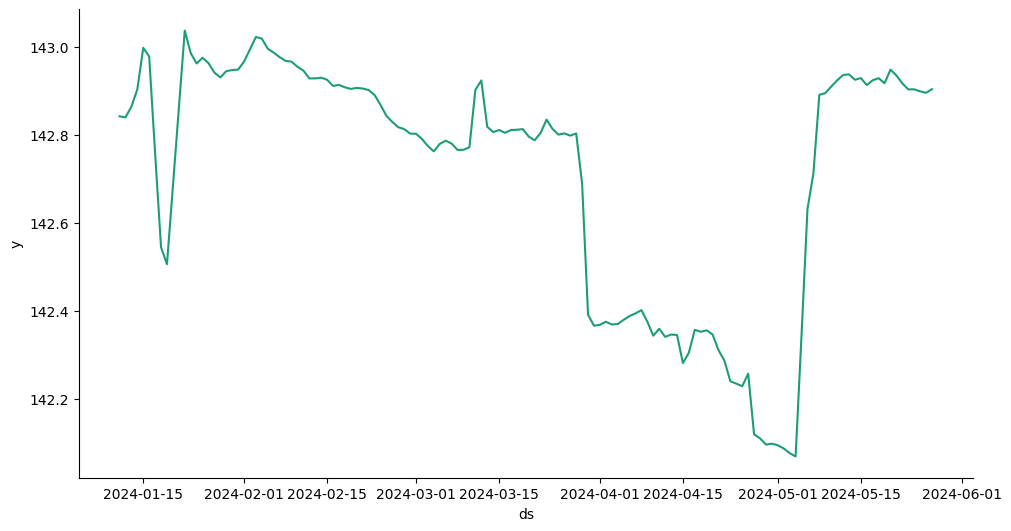
\includegraphics[width=\linewidth]{figures/No.3data} 
	
	% 替换为你的图片文件名
	%   \includegraphics[width=0.8\linewidth]{egfigure.eps}
	
	% 3号微波电子管的数据可视化,其中横坐标ds代表日期,纵坐标代表电流。可以看到,该微波电子管的数据具有较大的随机波动性。
	
	\caption{Visualization of Data for Component No.3. where the abscissa ds represents the date and the ordinate represents the current. It can be seen that the data of this microwave tube has large random fluctuations.}
	\label{fig:No3_original}
\end{figure}


\subsection{Dataset Description}
本实验的数据集,由小组成员采集于工业和信息化部电子第五研究所,采集对象为六个不同类型的电子元器件(分别是三号到八号),采集的数据为特定的条件下,持续时间内电子元件的电流大小与时间。本实验的训练集为四号电子原件,总共包含1058个时间步数据;而其他数据集,则用于测试和验证。

各个电子元件对应的时间序列数据,如下:
\begin{itemize}
    \item Component 3: 138 time steps.
    \item Component 5: 139 time steps.
    \item Component 6: 128 time steps.
    \item Component 7: 139 time steps.
    \item Component 8: 109 time steps.
\end{itemize}

每个电子元件对应一个数据集,包含电流随着时间的数值,及其对应的时间步。


\subsection{Data Preprocessing}

\begin{figure}[H]
	\centering
	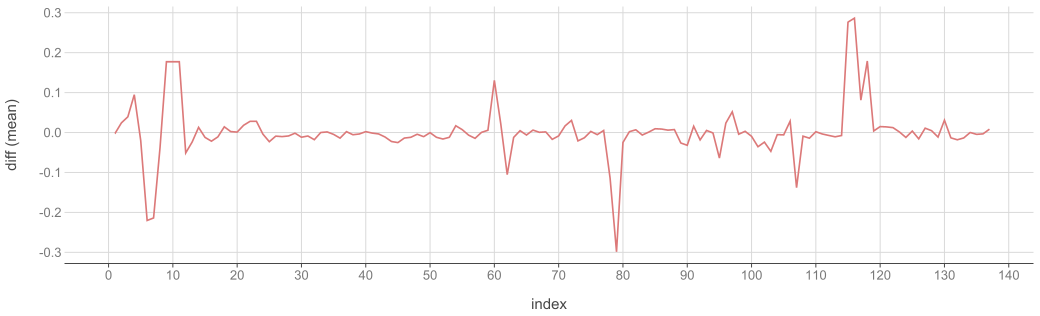
\includegraphics[width=\linewidth]{figures/No.3diff} 
	\caption{No.3 的时间序列数据的差分的可视化。图中每个点,代表原本数据集中的点与上一个点的差,反映了时间序列数据的随着时间将变化的程度。我们可以看到在发生突变的地方,对应的diff值都较大,而大部分的点都处在稍微比零更小的区域,符合元器件随着时间的变化,电流变小、寿命变短的情况}
	\label{fig:No3_diff}
	
\end{figure}


通过图\ref{fig:No3_original},我们可以看到,由于检测环境的限制,测出来的电流数值的时间序列数据,具有明显的突变,这很可能是由于实验环境(比如测电流时钳子的松动等)而导致的突变,而非电子原件本身的变化。为了能够学习到真正的时间序列数据模型,我们需要对原本的电流数值的时间序列数据进行一定的预处理。


接下来,我们将以3号电子元件为例子,介绍我们进行数据预处理的流程。

因为存在数值的突变(异常值),为了使得这部分异常值回归正常,我们需要对其进行差分处理(如图\ref{fig:No3_diff}所示)。经过差分之后可以看到,图中每个点,代表原本数据集中的点与上一个点的差,反映了时间序列数据的随着时间将变化的程度。发生突变的地方都对应着diff值较大的点;而大部分的点都处在稍微比零更小的区域,符合元器件随着时间的变化,电流变小、寿命变短的情况。

为了判断出哪些差分是不合理的(异常的),我们假设这些差分的分布符合正态分布。通过计算所有diff值的均值和方差,可以得到对应的正态分布(如图\ref{fig:No.3_Diff_and_Normal_Distribution}所示)。借助得到的正态分布,我们规定,将超过该正态分布95\%置信区间的diff值,视为异常值(见图\ref{fig:No.3_Abnormal_Value}),在后续的数据处理中进行剔除。我们利用得到的正态分布,随机模拟出一个更加合理的数值,并进行替换。

\begin{figure}[H]
	\centering
	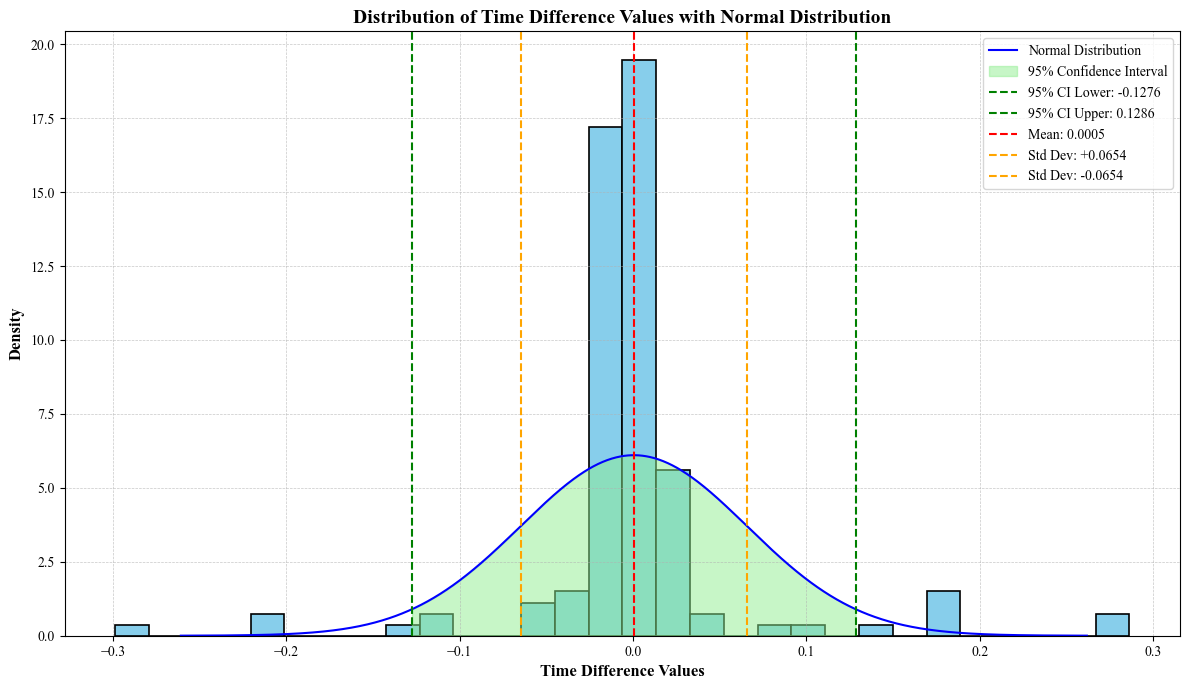
\includegraphics[width=\linewidth]{figures/No.3_Diff_and_Normal_Distribution} 
	\caption{电流时间序列的差分的频次分布 以及 对应的正态分布图。可以看到大部分diff数值集中在林附近的区域,上下波动,只有少数数值处在变化较大的区间。我们将超过置信区间95\%的数据视为异常数据,并在下一步的数据处理中进行处理}
	\label{fig:No.3_Diff_and_Normal_Distribution}
\end{figure}


\begin{figure}[H]
	\centering
	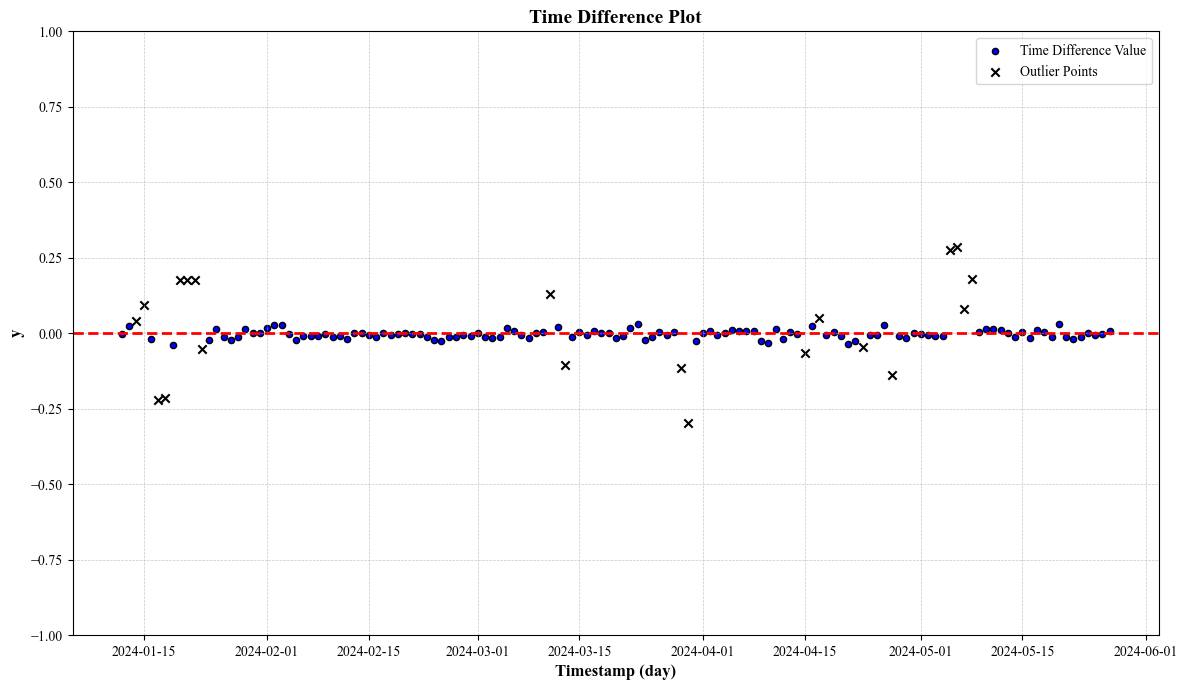
\includegraphics[width=\linewidth]{figures/No.3_Abnormal_Value} 
	\caption{电流时间序列的差分的频次分布 以及 对应的正态分布图。可以看到大部分diff数值集中在林附近的区域,上下波动,只有少数数值处在变化较大的区间。我们将超过置信区间95\%的数据视为异常数据,并在下一步的数据处理中进行处理}
	\label{fig:No.3_Abnormal_Value}
\end{figure}

经过预处理之后,不符合要求的异常值已经被替换为符合分布数值,该数值为随机数,且符合该正态分布(如图\ref{fig:No.3_Corrected_and_Normal_Distribution})。将其差分重新转换回电流数值的时间序列,即可得到处理过的数据(如图\ref{fig:No.3data_precessed})。对比图\ref{fig:No3_original}此时已经不再有突变的异常值了。

其余的电子管,都按照相同的流程进行处理,最终得到所有预处理的数据。并且,我们将使用4号管,作为训练集。利用其对模型进行微调,最终得到的模型,再进行迁移学习,预测其它各个管的电子元器件的寿命。

\begin{figure}[H]
	\centering
	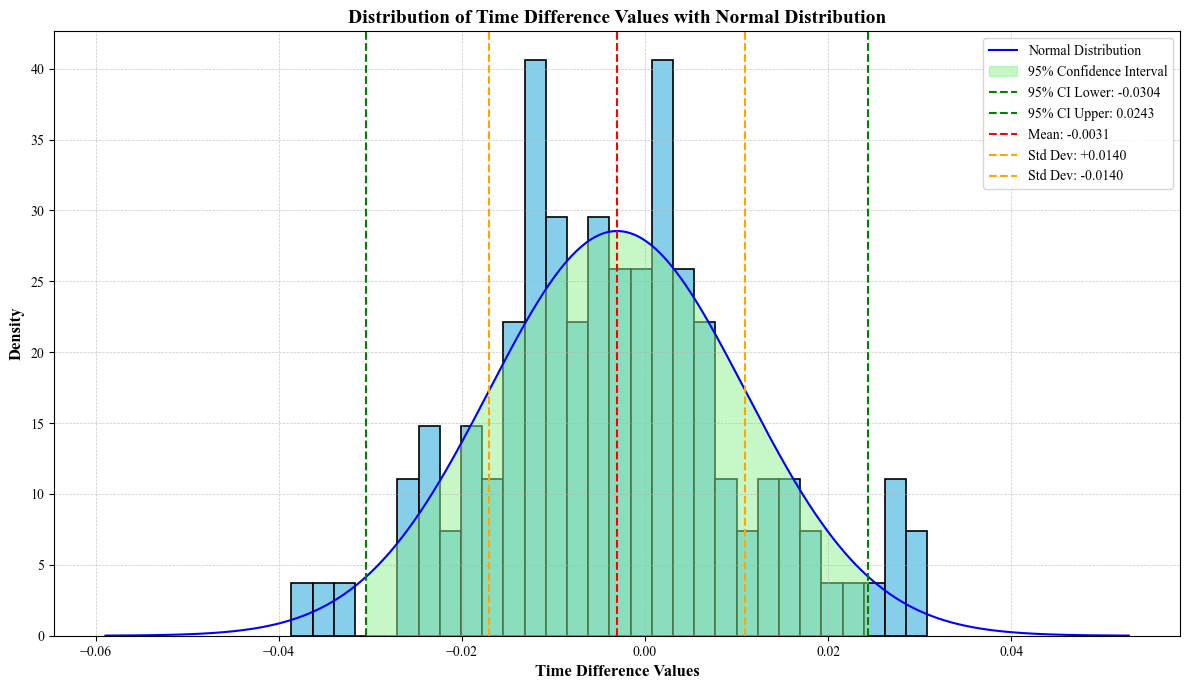
\includegraphics[width=\linewidth]{figures/No.3_Corrected_and_Normal_Distribution} 
	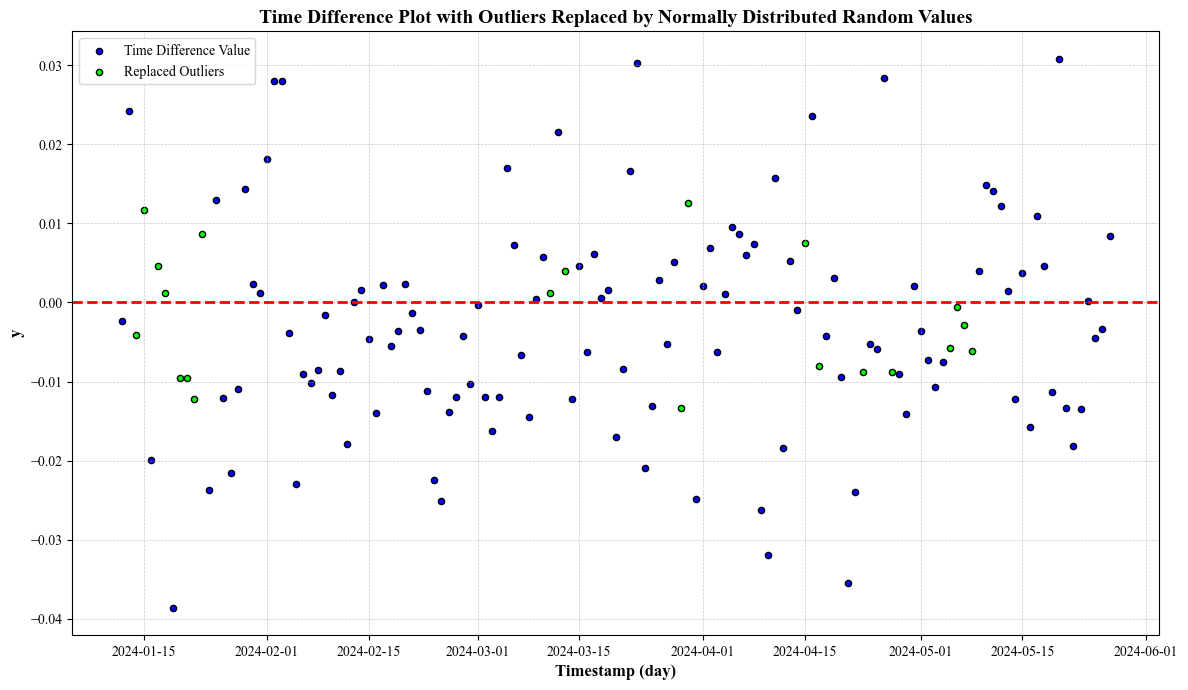
\includegraphics[width=\linewidth]{figures/No.3_Corrected_Diff} 
	\caption{Electronic components No.3 Correted difference and corresponding normal distribution.}
	\label{fig:No.3_Corrected_and_Normal_Distribution}
\end{figure}

\begin{figure}[H]
	\centering
	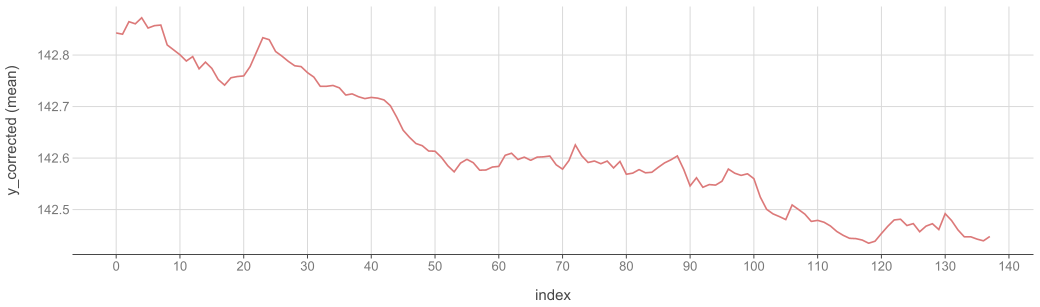
\includegraphics[width=\linewidth]{figures/No.3data_precessed} 
	\caption{Processed data about electronic components No.3.}
	\label{fig:No.3data_precessed}
\end{figure}
